%----------------------------------------
% Preamble to set up the document
%----------------------------------------
\documentclass{article}

% set up packages (you shouldn't need to touch this)
\usepackage{graphicx}  % required to insert images
\usepackage{hyperref}  % for hyperlinks
\usepackage[svgnames]{xcolor}  % to change hyperlink colors

\usepackage{float} 
\usepackage{listings}
\usepackage{lmodern}
\usepackage{xcolor}
\usepackage{comment}
\usepackage{color}
\usepackage{amsmath}
\usepackage{amsfonts}
\usepackage{amssymb}
\colorlet{linkcolour}{DarkBlue}
\hypersetup{colorlinks=true, linkcolor=linkcolour, citecolor=linkcolour, urlcolor=linkcolour,}

% Margins
\topmargin=-0.45in
\evensidemargin=0in
\oddsidemargin=0in
\textwidth=6.5in
\textheight=9.0in
\headsep=0.25in

% use a sans serif font
\renewcommand{\familydefault}{\sfdefault}

%----------------------------------------
% Step 1: Edit the lecture title
%----------------------------------------
\title{
Lecture 3: Computational Complexity \\  % Lecture title
Modeling Social Data, Spring 2019 \\   % Course title
Columbia University                    % School
}

%----------------------------------------
% Step 2: Edit your name and the date
%----------------------------------------
\author{Kiran Ramesh}                     % Scribe's name
\date{February 11, 2019}                % Lecture date

\begin{document}

\maketitle


%----------------------------------------
% Step 3:
% Rename uni.tex to match your uni,
% edit the filename accordingly below,
% and put your notes in this file
%----------------------------------------
%----------------------------------------
% Write your notes here
%----------------------------------------
\section{Introduction}
This lecture is about evaluating a research results. The main evaluation questions that one should ask are the following
\begin{enumerate}
  \item Was the research done and reported honestly / correctly?
  \item Is the result real or an artifact of the data / analysis?
  \item Will it hold up over time?
  \item How robust is the result to small changes?
  \item	How important / useful is the finding?
\end{enumerate}
\section{Reproducibility and Replicability}
We usually take the optimistic view that most researchers who publish their results are honest. However,some exceptions were reported, although few, in social science Literature available \href{https://en.wikipedia.org/wiki/List_of_scientific_misconduct_incidents#Social_sciences}{here}.

The two main criteria for evaluating credibility of a research is the reproducibility and replicability of the results. Reproducibility is the ability to independently verify the exact results using the same data and the same analysis. 
This is improving with better software engineering practices among researchers like

\begin{itemize}
  \item Literate programming(Jupyter,Rmarkdown)
  \item Automated build scripts
  \item Containers(Docker,Code Ocean)
\end{itemize}

The well renowned journals like NIPS started to encourage researchers by attaching acknowledgement badges on their published papers as shown in Figure 1. 

\begin{figure} [ht]
  \begin{center}
    
\includegraphics[width=0.5\textwidth]{figures/badges.png}
    \caption{
    NIPS Badges
      }
    \label{fig:badges}
  \end{center}
\end{figure}

Replicability is the question of whether the result holds up with new data under the same analysis. Since it's easy to be fooled by randomness, and Noise can dominate signal in small datasets and asking too many questions of the data can lead to overfitting.
Open science collaboration conducted replications of 100 experimental and correlation studies and deduced that 97 percent  had significant results, but 36 percent had statistically significant results, 47 percent of original effect sizes were in the 95 percent confidence interval of the replication effect size. This leads to a “Crisis” where one has to believe half of what he reads.

Figure 2 depicts the original study effect size versus replication effect size. 

\begin{figure}[ht]
  \begin{center}
    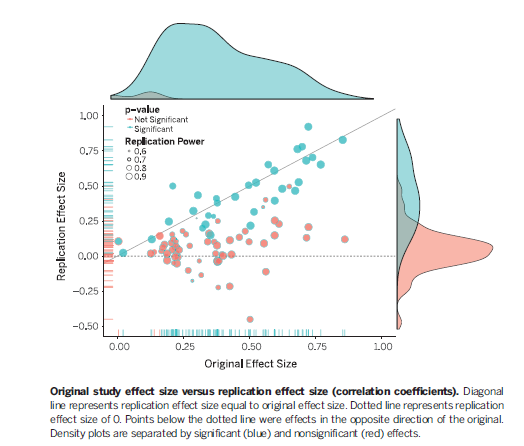
\includegraphics[width=0.5\textwidth]{figures/Crisis.png}
    \caption{
    Original study effect size vs replication effect size.
      }
    \label{fig:badges}
  \end{center}
\end{figure}

\section{Role of Statistics}
Then, we talked in class through three quizes about the role of statistics specifically the hypothesis testing, p-values, statistical significance, confidence intervals and effect sizes. We draw the below conclusion on the these quizes: 
\begin{enumerate}
  \item Quiz 1 : One should choose Treatment A , even if it is with small numbers of participants , because following the below formula: \begin{equation}
  {\sigma _{se}}={\sigma _{sd}}/ \sqrt{N}
\end{equation}
Under the same uncertainty about the mean ( standard error ) , the lower the N in the denominator of equation 1, the lower the standard deviation ( numerator of equation 1), as shown in Figure 3. 

\begin{figure}[ht]
  \begin{center}
    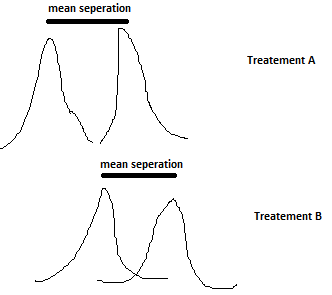
\includegraphics[width=0.5\textwidth]{figures/treatementA.png}
    \caption{
    Effect size
      }
    \label{fig:badges}
  \end{center}
\end{figure}
  

 \item Quiz 2 : All answers are false, the p-value given here is not a sufficient indicator of the null hypothesis, experimental hypothesis. 
 
 \item Quiz 3: Conclusion to draw here is one should not fool people with better visualization as it could be the case in Figure 4. 

 \begin{figure}[ht]
  \begin{center}
    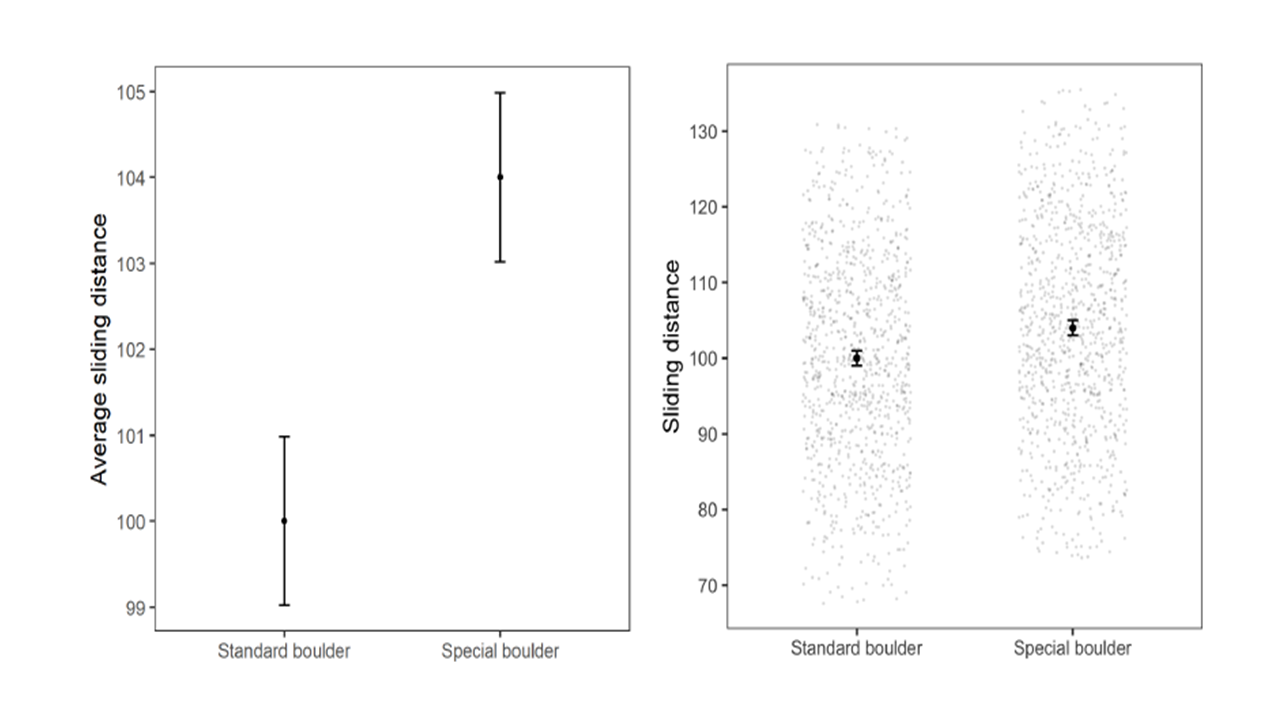
\includegraphics[width=0.5\textwidth]{figures/quiz3.png}
    \caption{
    Left: Bad visualization Right: Correct visualization
      }
    \label{fig:quiz3}
  \end{center}
\end{figure}

 
\end{enumerate}


\section{Some Statistics Thoughts...}
We cannot prove theories are right.Sometimes we can find contradictions to prove things false.Most often we have to settle for ruling things that are unlikely. How unlikely are my results in a boring world?  

Assuming boring world ( H0 is true) 
Imaging running study many times in a boring world as shown in Figure 5. 
Look at distribution of outcomes ( test statistics) from repetition in a boring world. ( Figure 6) . 
Compare outcome ( 100 flips ) from actual world to this distribution. For instance, if actual outcome is 0.61 , as shown in Figure 7, It is unlikely that we live in a boring world and thus one could reject the Null H0. 
However, if actual outcome is 0.52, as shown in Figure 8 one cannot reject the Null. And thus the world could be boring. 

As a conclusion :
\begin{enumerate}
\item One need to put a threshold on the p-value
\item  Need to quantify Unlikeliness. 
\end{enumerate}


P-value tells you probability of data you saw given that you are in a boring world. ( Null H0 is True) 
 \begin{equation}
  p(D/H_{0} True)
\end{equation}

You have to decide for p-value on a threshold alpha below which you reject boring world. 
 \begin{equation}
  \alpha
\end{equation} 
Alpha is false positive rate and the convention value is 0.05 (1 in 20) 
\begin{equation}
\alpha= p( reject H_{0}/H_{0} true)
\end{equation}
But what about 
\begin{equation}
p( reject H_{0}/H_{0} false)
\end{equation} 

\begin{itemize}
\item Assume exciting world where effect exists ( H0 is false )
\item Run a study in exciting world many times, execute test and look how often to reject the Null as in Figure 9.Convention: Want power about 80 % 

\begin{figure}[ht]
  \begin{center}
    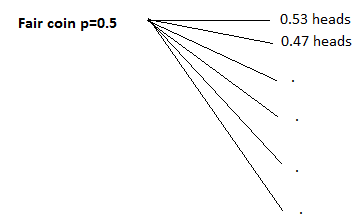
\includegraphics[width=0.5\textwidth]{figures/fig5.png}
    \caption{
    Boring world ( H0 is true) 
      }
    \label{fig:fig8}
  \end{center}
\end{figure}

 \begin{figure}[ht]
  \begin{center}
    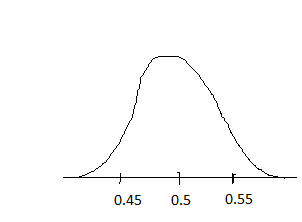
\includegraphics[width=0.5\textwidth]{figures/fig6.png}
    \caption{
    Distribution of outcomes from repetition in a boring world
      }
    \label{fig:fig5}
  \end{center}
\end{figure}

 \begin{figure}[ht]
  \begin{center}
    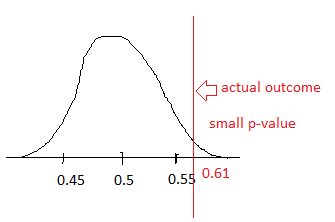
\includegraphics[width=0.5\textwidth]{figures/fig7.png}
    \caption{
    Reject the Null H0
      }
    \label{fig:fig6}
  \end{center}
\end{figure}

\begin{figure}[ht]
  \begin{center}
    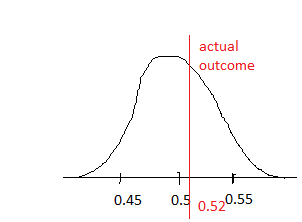
\includegraphics[width=0.5\textwidth]{figures/fig8.png}
    \caption{
    Cannot Reject the Null H0
      }
    \label{fig:fig7}
  \end{center}
\end{figure}

\begin{figure}[ht]
  \begin{center}
    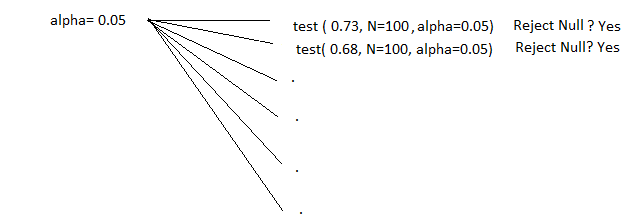
\includegraphics[width=0.5\textwidth]{figures/fig9.png}
    \caption{
    Study run in an exciting world with alpha=0.05 
      }
    \label{fig:fig9}
  \end{center}
\end{figure}

\end{itemize}







\end{document}

%%% Local Variables:
%%% mode: latex
%%% TeX-master: t
%%% End:
